% Chapter Template

\chapter{Introduction} % Main chapter title

\label{ChapterIntroduction}

%----------------------------------------------------------------------------------------
%	SECTION 1
%----------------------------------------------------------------------------------------

\section{Introduction to Cryptography}
The terms \emph{Cryptography}, from the Greek \emph{krypt\`os} (secret) and \emph{graphein} (writing), and \emph{Cryptanalysis}, denotes two branches of a science named \emph{Cryptology}, or \emph{science of the secret}. Cryptography initially refers to the art of \emph{encrypting} messages, which means writing meaningful messages in such a way to appear nonsense to anyone unaware of the encryption process. The readable message is referred to as \emph{plaintext}, while the unintelligible output of the encryption is referred to as \emph{ciphertext}. In general, cryptography aims to construct protocols to secure communication, while cryptanalysis studies the resistance of cryptographic techniques, developing \emph{attacks} to break the cryptosystems' security claims. These two complementary domains evolve in parallels, since the evolution of attack techniques allows conceiving more resistant cryptographic algorithms, and inversely the resistance of such algorithms requires the conception of more sophisticated attacks.\\

The art of cryptography is very ancient, probably as ancient as the language, but only the development of information technology made cryptology take the shape of a proper science, sometimes referred to as \emph{Modern Cryptology}. The last is seen as a branch of different disciplines, such as applied mathematics, computer science, electrical engineering, and communication science. Modern cryptosystems exploit algorithms based on mathematical tools and are implemented as computer programs, or electronic circuits. Their goal is to provide security functionalities for communications that use \emph{insecure channels}, for example the internet. In particular, modern cryptosystems are designed in order to ensure at least one of the four following information security properties:
\begin{itemize}
\item[a.] \emph{confidentiality}: the transmitted message must be readable only by a chosen pool of authorized entities;
\item[b.] \emph{authenticity}: the receiver can verify the identity of the sender of a message;
\item[c.] \emph{non-repudiation}: the sender of a message cannot deny having sent the message afterwards;
\item[d.] \emph{data integrity}: the receiver can be convinced that the message has not been corrupted during the transmission.


\end{itemize} 

Two branches of cryptography may be distinguished: the \emph{symmetric cryptography} and the \emph{asymmetric cryptography}. The first one historically appeared before and is based on the hypothesis that the two communicating entities share a common secret, or private key; for this reason this is also called \emph{secret key cryptography}. The second one, introduced around 1970, allows any entity to encrypt a message in such a way that only a unique chosen other entity could decrypt it; this is also called \emph{public key cryptography}. \\

A general principle in cryptography, nowadays widely accepted by cryptography researchers, is the one given by Kerckhoff in 19th century: it states that cryptosystems should be secure even if everything about the system, except the key, is public knowledge. Following this principle, today many industrials and governmental agencies exploit for their security services cryptosystems based over standardized algorithms. Such algorithms are of public domain, thus have been tested and tried to be broken by a large amount of people, before, during and after the standardization process. Resistance to many attempts of attacks is actually the strengths of standard algorithms.\\

In the following part of this section a description of the two standard cryptographic primitives, \emph{i.e.} building block algorithms used to build cryptographic protocols, that will be often cited in this thesis is provided; a symmetric one, the AES, and an asymmetric one, the RSA. 
\subsection{Description of AES}
The \emph{Advanced Encryption Standard} (AES) has been standardized in 2001 by the United States governmental agency \emph{National Institute of Standards and Technology} (NIST) through the \emph{Federal Information
Processing Standards Publication 197 } (FIPS PUB 197) \cite{nist197}. It is a symmetric \emph{block cipher}, \emph{i.e.} an algorithm operating on fixed-length groups of bits.\footnote{in contrast with \emph{stream ciphers}, which operate over a single plaintext bit at time} The AES operates on blocks of 128 bits of plaintext, and can use keys of size 128, 192 or 256 bits. The encryption is done by rounds. The number of executed rounds depends on the key size (10 rounds for 128 bits, 12 for 192 and 14 pour 256). The basic unit for processing in the AES algorithm is a byte. For AES internal operations, bytes are arranged on a two-dimensional array of bytes called the \emph{state}, denoted $s$. Such a state has 4 rows and 4 columns, thus contains 16 bytes. The byte lying at the $i$-th row, $j$-th column of $s$ will be denoted by $s_{i,j}$ for $i,j\in\{0,1,2,3\}$. The 16 input bytes and the 16 output bytes are indexed column-wise as shown in Fig.~\ref{fig:AES_state}. Each element $s_{i,j}$ of a state is mathematically seen as an element of the \emph{Rjindael finite field}, defined as $GF(2^8) = \mathbb{Z}/{2\mathbb{Z}[X]}/P(X)$ where $P(X) = X^8 + X^4 + X^3 + X + 1$. Five functions are performed during the AES, named KeySchedule, AddRoundKey, SubBytes, ShiftRows and MixColumns. At high level the AES algorithm is described hereafter:
\begin{itemize}
\item[]\textbf{Key Expansion:}  derivation of round keys from secret key through the KeySchedule function
\item[]\textbf{Round 0:}  
\begin{itemize}
\item[] AddRoundKey
\end{itemize}
\item[] \textbf{Rounds 1 to penultimate:}
\begin{itemize}
\item[] SubBytes
\item[] ShiftRows
\item[] MixColumns
\item[] AddRoundKey
\end{itemize}
\item[] \textbf{Last Round:}
\begin{itemize}
\item[] SubBytes
\item[] ShiftRows
\item[] AddRoundKey
\end{itemize}
\end{itemize}

\begin{figure}
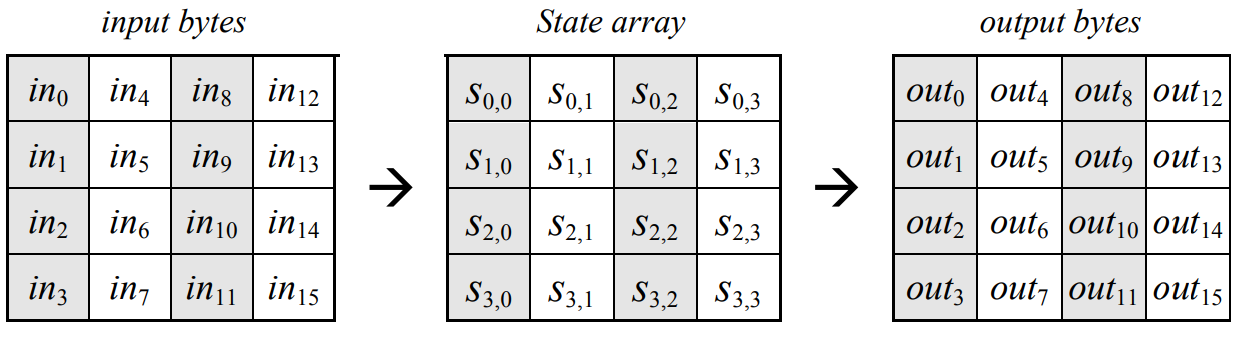
\includegraphics[width = \textwidth]{../Figures/FISP_AES/state.png} 
\caption[State array input and output.]{State array input and output. Source: \cite{nist197}.}\label{fig:AES_state}
\end{figure}

A description of the five functions is provided hereafter.

\subsubsection*{KeySchedule}
The key round of the initial round of AES coincides with the secret encryption key $\boldsymbol{K} = (k_{0,0},k_{0,1},\dots,k_{0,3}, k_{1,0},\dots,k_{1,3},\dots,k_{3,3})$. The $i$-th round key is given by 
\begin{equation*}
\boldsymbol{K_i} = (k_{4i,0},k_{4i,1},\dots,k_{4i,3}, k_{4i+1,0},\dots,k_{4i+1,3},\dots,k_{4i+3,3}),
\end{equation*}
where, for $i>3$
\begin{equation*}
\begin{cases}
k_{a,b} = k_{a-4,b}\oplus k_{a-1,b} & \mbox{if } a \not\equiv 0 \mbox{ mod } 4\\
k_{a,b} = k_{a-4,b}\oplus \Sbox(k_{a-1,(b+1) \mbox{mod } 4}) \oplus \mathrm{Rcon}(a) & \mbox{if } a \equiv 0 \mbox{ mod } 4 \mathrm{,}
\end{cases}
\end{equation*}

where $Rcon(a) = \{02\}^{a-1}$ in the Rjindael finite field.\footnote{where $\{02\}=(00000010)_2$ is represented by the polynomial $x$}

\subsubsection*{AddRoundKey} Each byte of the State is combined with the corresponding byte of the round key via an addition over the Rjindael field $GF(2^8)$, \ie a bitwise exclusive OR (\emph{XOR}) operation $\oplus$.
\subsubsection*{SubBytes}
\begin{figure}
\centering
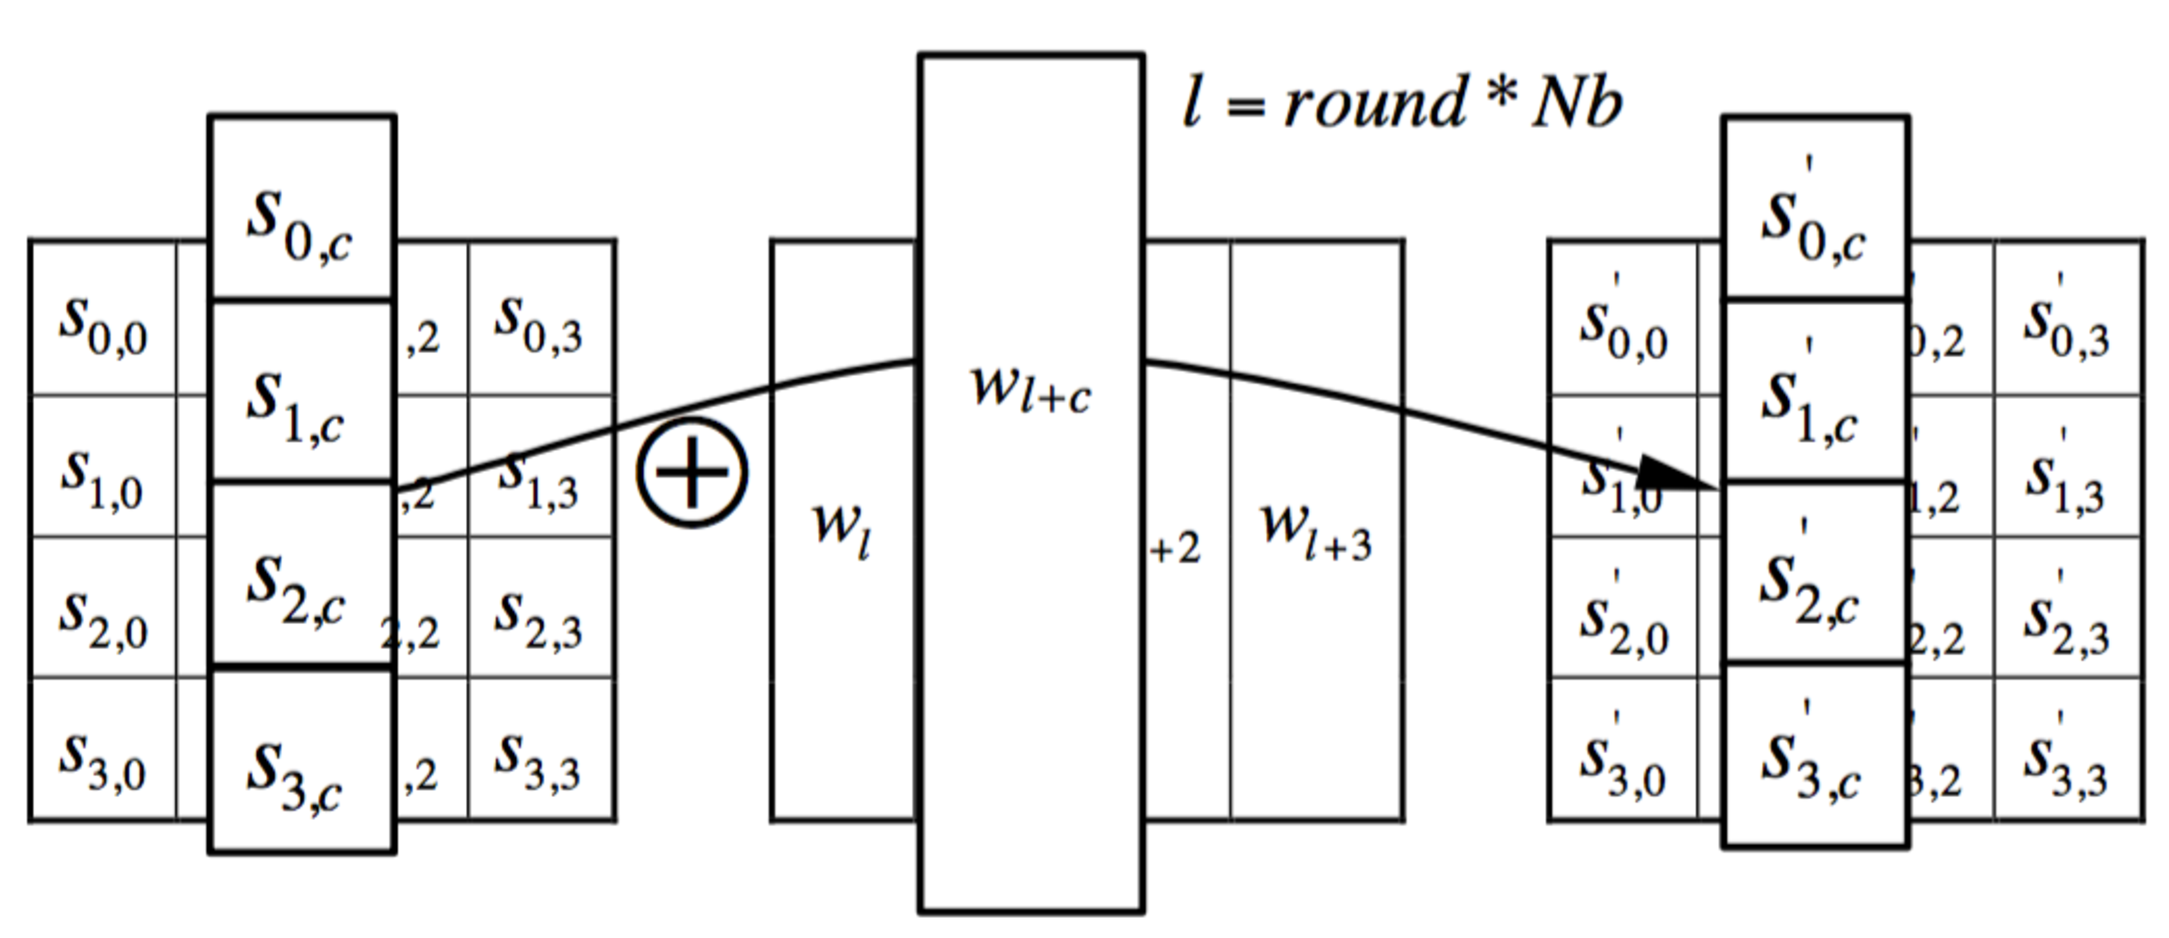
\includegraphics[width = .60\textwidth]{../Figures/FISP_AES/add_round_key.pdf} 
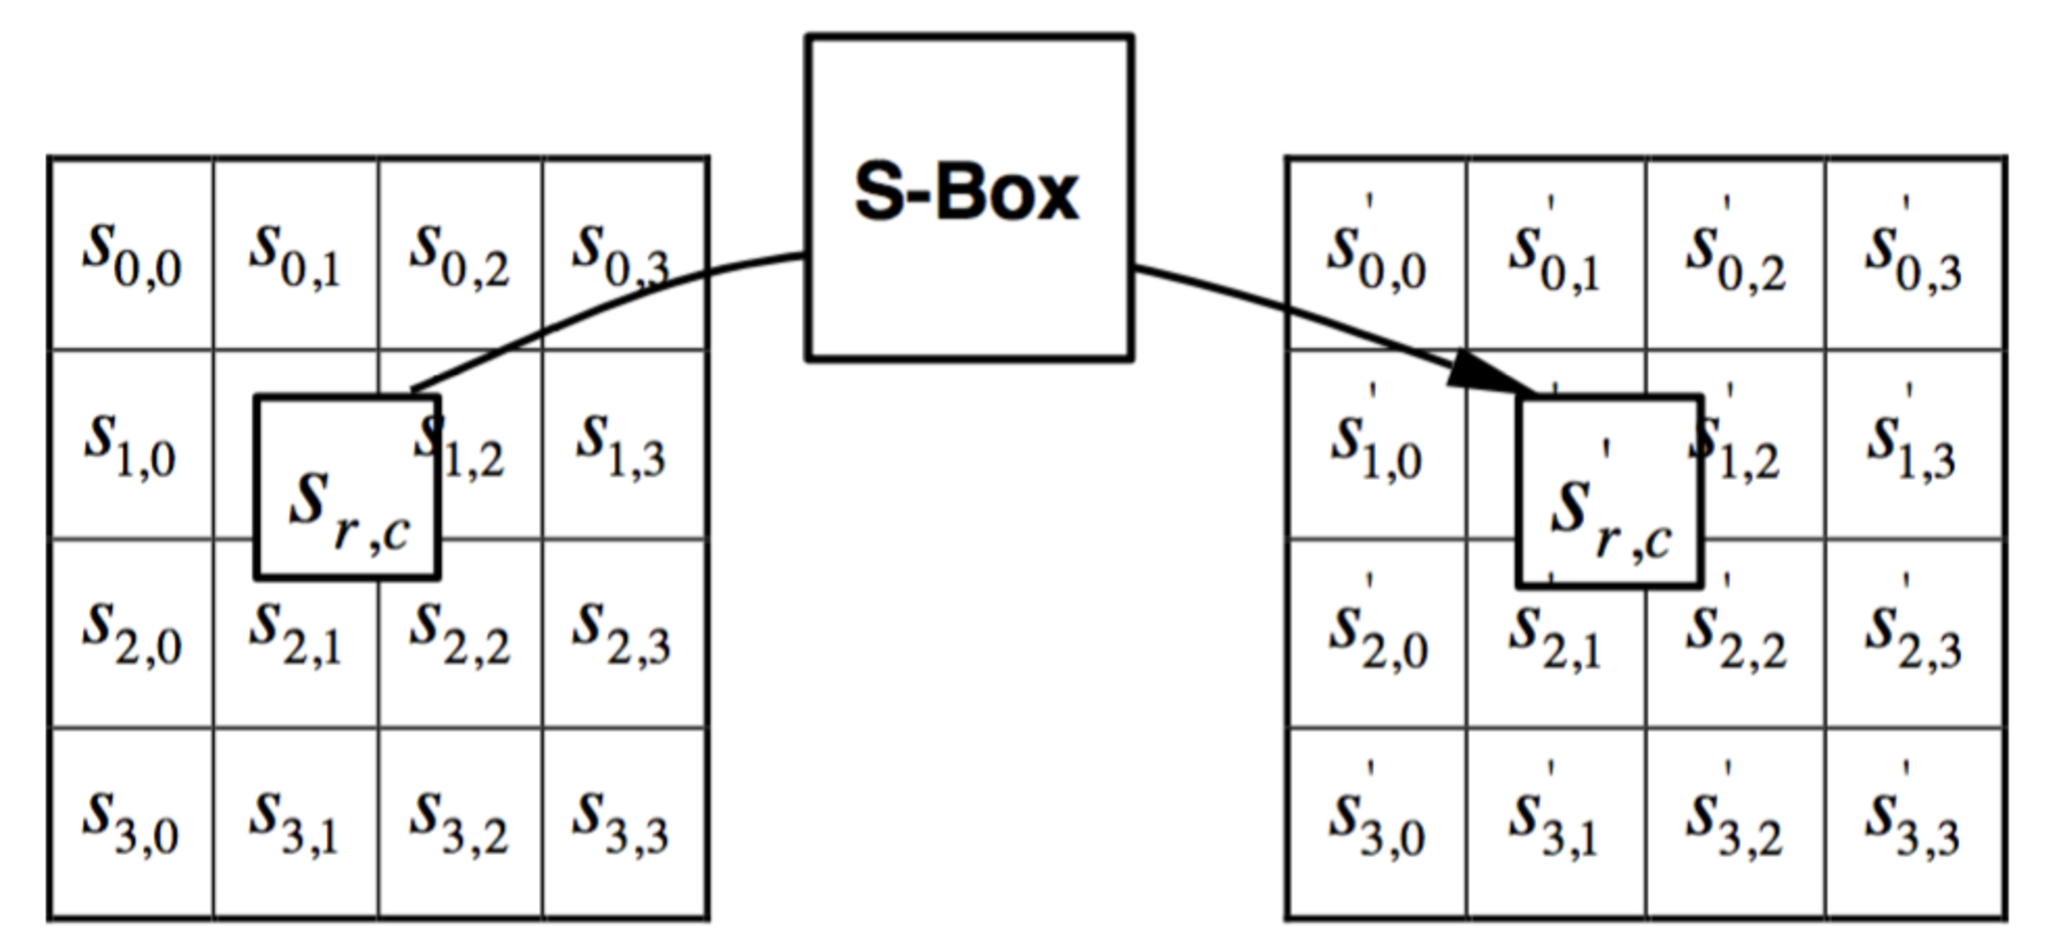
\includegraphics[width = .45\textwidth]{../Figures/FISP_AES/sbox.pdf} 
\caption[AddRoundKey and SubBytes.]{AddRoundKey (top) and SubBytes (bottom) operate over the State byte by byte, independently. Source: \cite{nist197}.}\label{fig:AES_sbox}
\end{figure}
The SubBytes transformation is a non-linear byte invertible substitution that operates independently on each byte of the State using a substitution table (called \emph{S-Box}). The SubBytes is composed of the following two functions:
\begin{itemize}
\item the inversion in $GF(2^8)$ where the element $\{00\}$ is mapped to itself
\item the affine transformation which maps each byte $b_i$ to:
\begin{equation}
b_i \oplus b_{(i+4)\mbox{mod }8} \oplus b_{(i+5)\mbox{mod }8} \oplus b_{(i+6)\mbox{mod }8} \oplus b_{(i+7)\mbox{mod }8} \oplus c_i \mbox{ ,}
\end{equation}
 where $c_i$ is the $i^\text{th}$ bit of $\{63\}  = (01100011)_2$.
\end{itemize}  
\subsubsection*{ShiftRows}
The bytes in the last second, third and fourth rows of the State are cyclically shifted over 1, 2, and 3 bytes respectively.
\subsubsection*{MixColumns}
Each column of the State is treated as a four-term polynomial. They are considered as polynomials over the Rjindael field $GF(2^8)$ and multiplied modulo $X^4 +1$ with a fixed polynomial $a(X) = \{03\}X^3 +\{01\}X^2 + \{01\}X + \{02\}$.

\begin{figure}
\centering
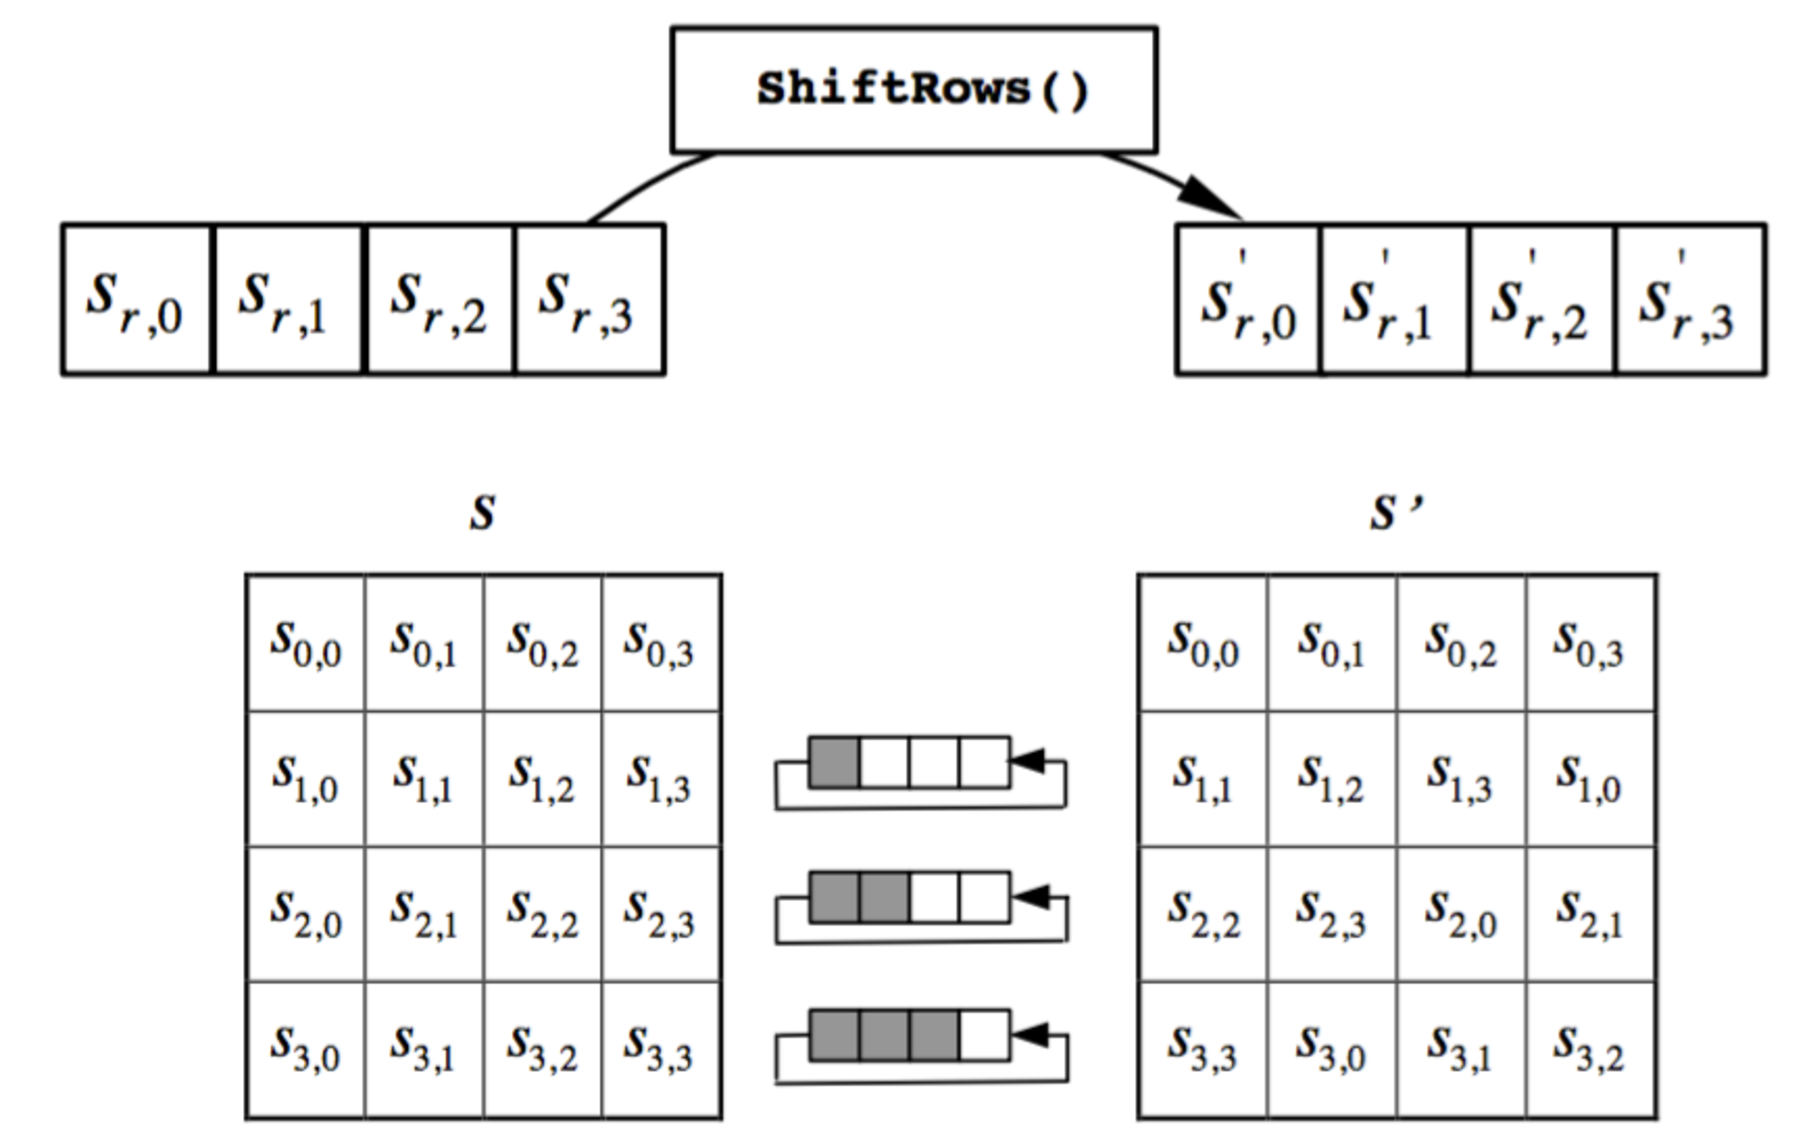
\includegraphics[width = .45\textwidth]{../Figures/FISP_AES/shift_rows.pdf} 
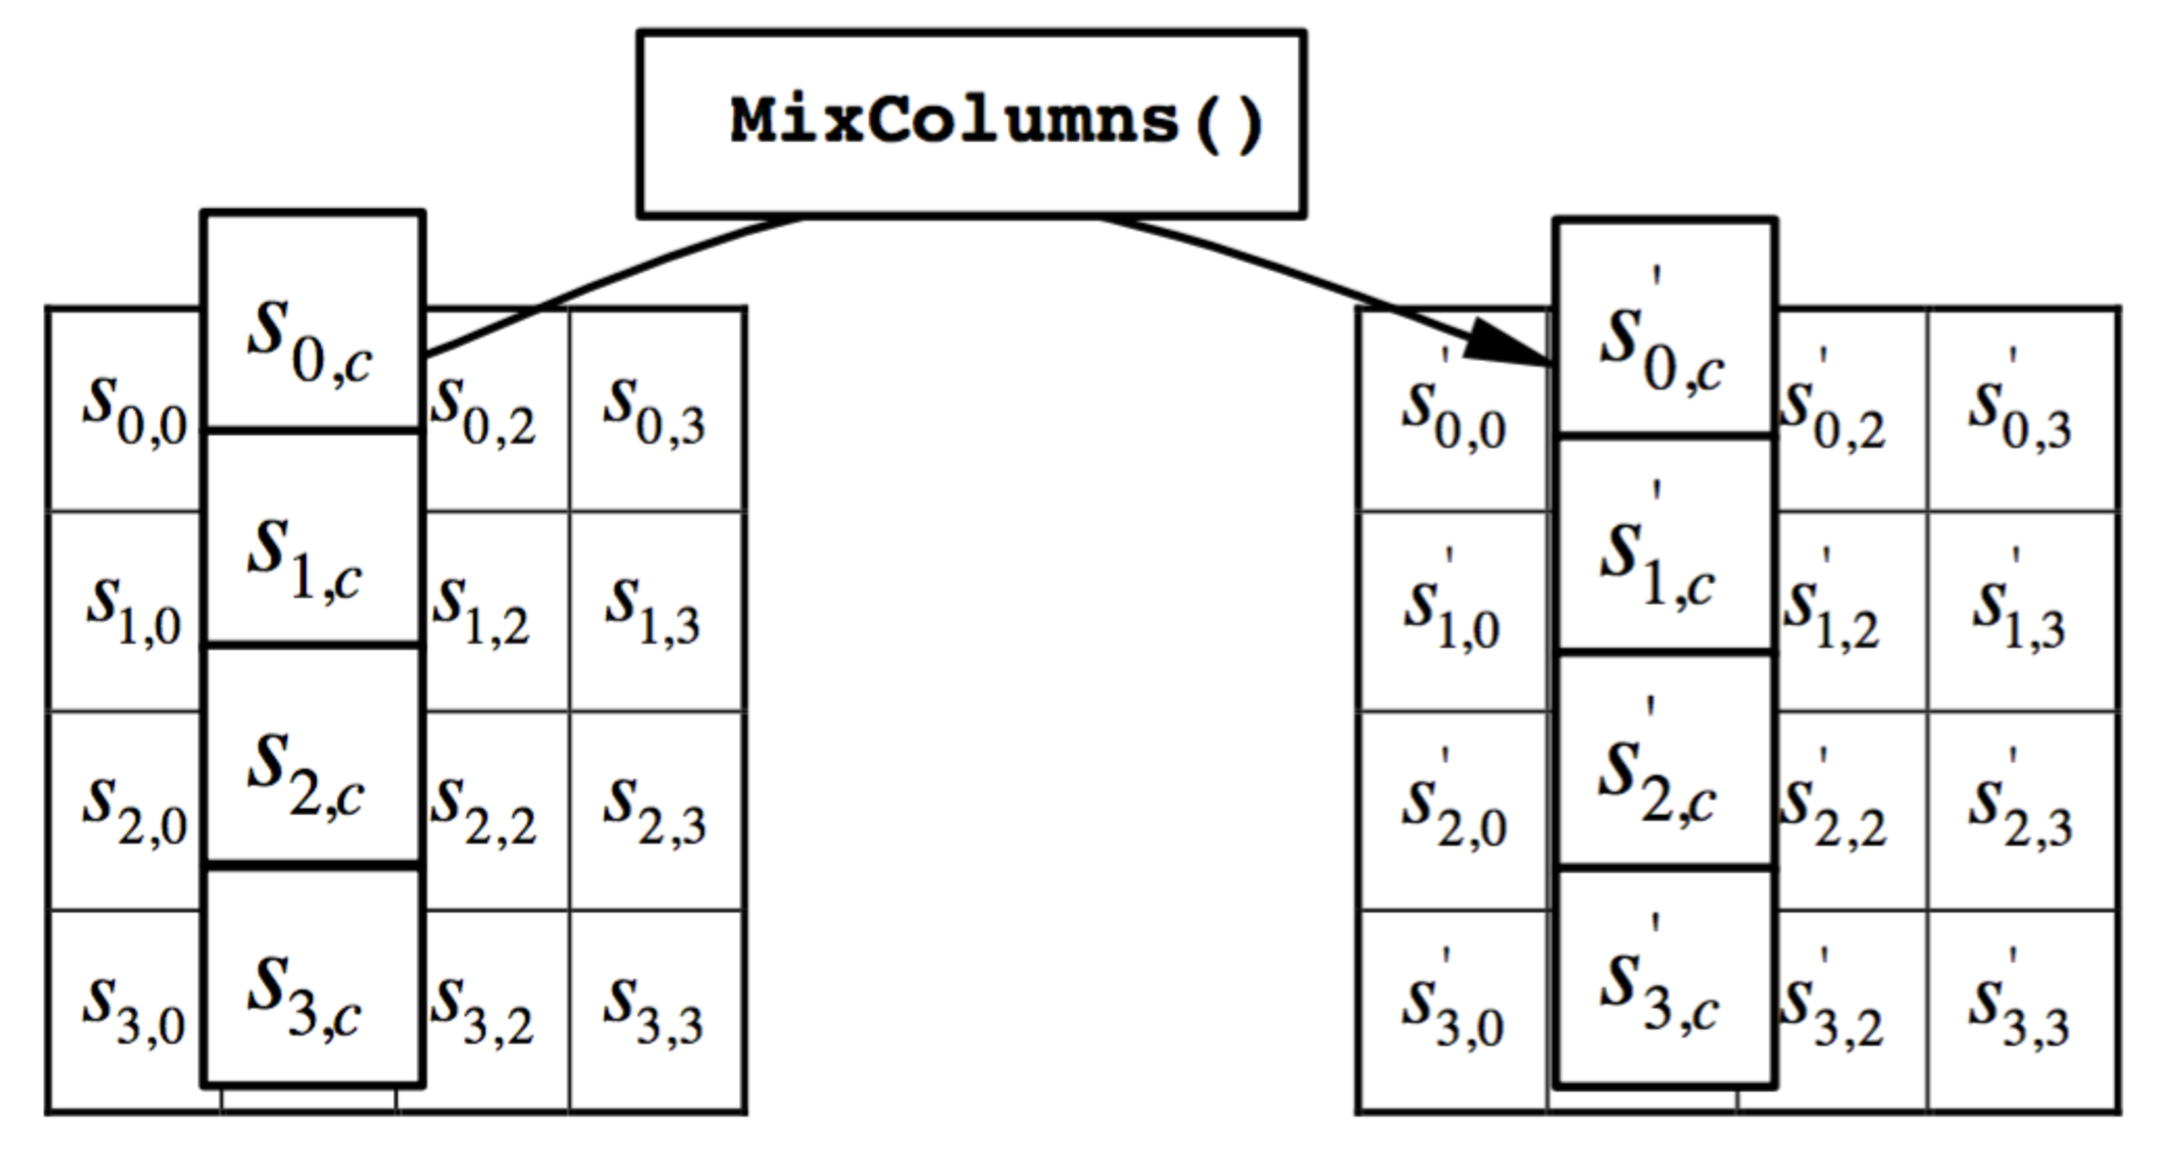
\includegraphics[width = .45\textwidth]{../Figures/FISP_AES/mix_columns.pdf} 
\caption[ShiftRows and MixColumns.]{ShiftRows operates over the State rows. MixColumns operates over the State columns. Source: \cite{nist197}.}\label{fig:AES_sbox}
\end{figure}

\subsection{Description of RSA}
The RSA cryptosystem, proposed in 1978 by Rivest, Shamir and Adleman \cite{rivest1978method}, represents the first practical realization of the use of trapdoor functions to provide asymmetric cryptography (a concept proposed two years earlier by Diffie, Helman and Merkle \cite{diffie1976new}). RSA is one of the most deployed, analysed, challenged, and discussed cryptosystems of all times, the seminal paper \cite{rivest1978method} counting today 18950 citations.\footnote{From Google Scholar, visited on January 2018.}\\

Hereafter a simplified description of the RSA algorithm is provided.\\
Let $N = p \times q$ be the product of two large primes of about the same size. Then we can compute two values $e,d$ such that $d = e^{-1} (\mbox{mod } \varphi(N))$, where $\varphi(N) = (p-1)\times(q-1)$ is the Euler's totient function of $N$, corresponding to the size of the multiplicative field $	\mathbb{Z}^\star_N$. The pair $(N,e)$ is the public key, and $d$ is the private one. Let $M \in	\mathbb{Z}^\star_N$ be a message. $M$ can be encrypted by computing the value $C = M^e (\mbox{mod } N)$. The ciphertext $C$ can then be decrypted by computing $C^d (\mbox{mod } N)$. The fact that the two transformations are mutually inverse is a consequence of the Euler's totient theorem. 
As $e$ denotes the public exponent, and $d$ the private one, the transformation $C = M^e (\mbox{mod } N)$ is called encryption as only the owner of the private key can retrieve the initial message. On the other hand $S = M^d (\mbox{mod } N)$ is called signature as it only needs public parameters to retrieve the initial message and thus anyone can verify that the owner of the private key has \emph{signed} $M$. The security of such a cryptosystem is based on the big integers factorization problem.


%----------------------------------------------------------------------------------------
%	SECTION 2
%----------------------------------------------------------------------------------------
\section{Secured Components}

As we have seen in the previous section, modern cryptography proposes solutions to secure communications that ask for electronic computations and repose their security over some secret keys. Keys are represented as long bit strings, impossible to be memorized by users. Thus, keys need to be stored in a secure medium, and never delivered in clear over insecure channels. Smart cards were historically conceived as a practical solution to such a key storage issue: they consist in small devices a user can easily carry around with, which not only store secret keys, but also are able to internally perform cryptographic operations, in such a way that keys are never asked to be delivered. The registrations of a first patent by Roland Moreno in 1974 and of a second one by Michel Ugon in 1977 are often referred to date the smart card invention, finally produced for the first time in 1979. Smart cards are pocket-sized plastic-made cards equipped with a secured component, which is typically an integrated circuit containing some computational units and some memories.\\

Today, about 40 years after its invention, they still have a huge diffusion, both in terms of applicative domains and in terms of quantity of exemplars. Indeed, they serve as credit or ATM cards, healthy cards, ID cards, public transport payment cards, fuel cards, identification and access badges, authorization cards for pay television, etc. Slightly changing the card support, we find other applications of the same kind of integrated circuits, for example the  mobile phone SIMs (\emph{Subscriber Identity Module}) and the electronic passports. In terms of quantity, it seems that in 2014 8.8 billion smart cards have been sold, \emph{i.e.} the same order of magnitude of the global population. \\

In addition to smart cards, the recent growing and variation of security needs lead to the development and specification of other kinds of secured components, for example the \emph{Trusted Execution Environment} (TEE), which as a secured part of the main processor of a smartphone or tablet, and the \emph{Trusted Platform Module} 
(TPM), which is a secure element providing cryptographic functionalities to a motherboard. 

\subsection{Embedded Cryptography Vulnerabilities}\label{sec:vulnerabilities}
\subsubsection{Side-Channel Attacks}
Until the middle of nineties, the security of embedded cryptosystems was considered as equivalent to the mathematical security of the cryptographic algorithm. In classical cryptanalysis an attacker has usually the knowledge of the algorithm (in accordance to the Kerckhoff's principle) and of some inputs and/or outputs. Starting from this data, his goal is to retrieve the secret key. This attack model considers the algorithm computation as a black box, in the sense that no internal variable can be observed during execution, only inputs and/or outputs. With his seminal paper about Side-Channel Attacks (SCAs) in 1996, Paul Kocher showed that such a black-box model fails once the algorithm is implemented over a material component \cite{kocher1996timing}: an attacker can indeed inspect its component during the execution of the cryptographic algorithm, monitor some physical quantities, for example the execution time \cite{kocher1996timing} or the instantaneous power consumption \cite{kocher1999differential} and deduct information about internal variables of the algorithm. Depending on the attacked algorithm, making inference over some well chosen internal variable (the so-called \emph{sensitive variables} of the algorithm) is sufficient to retrieve the secret key. After these first works it was shown that other observable physical quantities contained \emph{leakages} of sensitive information, for example the electromagnetic radiation emanating from the device \cite{gandolfi2001electromagnetic,quisquater2001electromagnetic} and the acoustic emanations \cite{genkin2014rsa}. Moreover, if until few years ago it was thought that only small devices, equipped with slow microprocessors and in a small-sized architecture, such as smart cards were vulnerable to this kind of Side-Channel Attacks, the last cited recent work about acoustic emanations, together with other works exploiting electromagnetic fluctuations pointed out that much faster and bigger devices, \emph{i.e.} laptops and desktop computers, are vulnerable as well \cite{genkin2015stealing,genkin2015get,genkin2016ecdh}.

\subsubsection{A Classification of the Attacks to Secured Components}\label{sec:classification_attacks}
\begin{table}[]
\centering
\caption{Classification of Attacks}
\label{fig:classification_attacks}
\begin{tabular}{|l|lll}
\cline{1-3}
\multirow{4}{*}{\textbf{Hardware Attacks}} & \multicolumn{1}{l|}{Passive} & \multicolumn{1}{l|}{Active} &                                    \\ \cline{2-4} 
                                           & \multicolumn{1}{l|}{}        & \multicolumn{1}{l|}{}       & \multicolumn{1}{l|}{Invasive}      \\ \cline{2-4} 
                                           & \multicolumn{1}{l|}{}        & \multicolumn{1}{l|}{}       & \multicolumn{1}{l|}{Semi-Invisive} \\ \cline{2-4} 
                                           & \multicolumn{1}{l|}{SCAs}    & \multicolumn{1}{l|}{FAs}    & \multicolumn{1}{l|}{Non-Invasive}  \\ \hline
\textbf{Software Attacks}                  &                              &                             &                                    \\ \cline{1-1}
\end{tabular}
\end{table}

The Side-Channel Attacks outlined in previous paragraph, and which are the main concern of this thesis,  belong to a much bigger family of attacks that can be performed to break cryptographic devices security claims. First of all software attacks and hardware attacks must be distinguished. Software attacks only exploit vulnerability coming from the way the component's code is written. Hardware attacks are still commonly classified on the base of two criteria: on one hand we can distinguish passive and active attacks, on the other hand we can distinguish invasive, semi-invasive, non-invasive attacks. 
\begin{itemize}
\item[] \textbf{Passive attacks:} in passive attack, the device is let run respecting its specifications. The attacker observes its behaviour without provoking any alteration;
\item[] \textbf{Active attacks:}  in active attacks a special manipulation is performed in order to make the normal behaviour of the device change. 
\end{itemize}


\begin{itemize}
\item[] \textbf{Invasive attacks}: in invasive attack, the device is depackaged and inspected at the level of the components technology. The circuit can be modified, broken, signals can be accessed via a probing station, etc. There is no limits to the manipulations attacker can do to the components;
\item[] \textbf{Semi-invasive attacks}: as in invasive attacks the device is depackaged, but in contrast to them, no direct electrical contact to the chip is done;
\item[] \textbf{Non-invasive attacks}: in non-invasive attacks the device is not modified and only accessible interfaces are exploited. 

In literature, the term Side-Channel Attacks commonly denotes the passive non-invasive attacks. In the same way, active non-invasive attacks are often referred to as \emph{Fault Injection Attacks}. 

\end{itemize}

\subsection{Certification of a Secure Hardware - The Common Criteria}
\begin{figure}
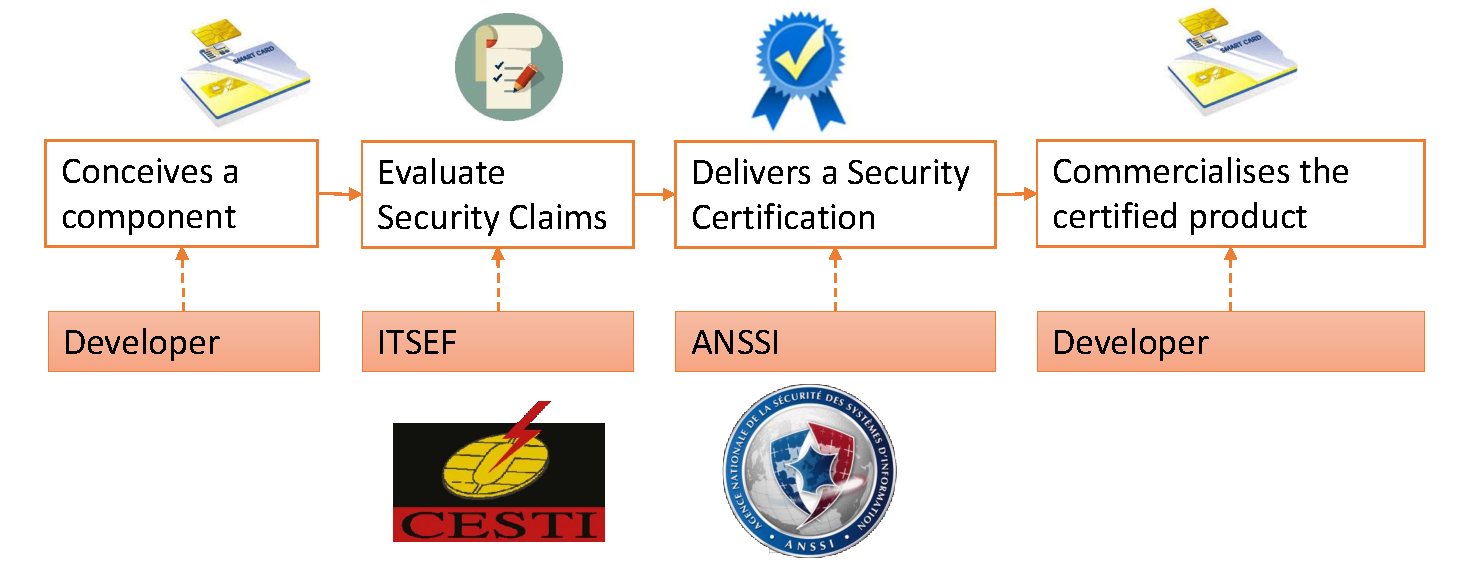
\includegraphics[width=\textwidth]{../Figures/ITSEF_ANSSI2.pdf} 
\caption{The actors of French Certification Scheme}
\end{figure}
In previous paragraphs we have evoked the great diffusion of the cryptographic devices, which implies consequent great risks in case of vulnerabilities of such largely diffused devices, and the existence of a wide range of attacks exploiting vulnerabilities coming from the way cryptography is embedded. These factors justify the importance and necessity to ensure reliability on the security claims of commercialised secured components and thus the arise of several guidelines and standards for their evaluation. The international standard ISO/IEC 15408, also known as \emph{Common Criteria for Information Technology Security Evaluation} (abbreviated as \emph{Common Criteria} or simply \emph{CC}) represents one of the stronger efforts in standardization, unifying in 1999 three previously existing standards:
\begin{itemize}
\item the \emph{Trusted Computer System Evaluation Criteria} (TCSEC - United States - 1983)
\item the \emph{Information Technology Security Evaluation Criteria} (ITSEC - France,Germany, Netherlands, United Kingdom - 1990)
\item the \emph{Canadian Trusted Computer Product Evaluation Criteria} (CTCPEC - Canada - 1993).
\end{itemize}

\subsubsection{The actors} The CC define four actors of the evaluation process of a secured component:
\begin{itemize}
\item \textbf{The Developer}, who conceives a product and wishes to sell it as a certified secured product. He sends a request for evaluation to the certification body and, once the request is accepted, he contacts an evaluation laboratory
\item \textbf{The ITSEF} is the \emph{IT Security Evaluation Facility}; in France it is named \emph{Centre d'Evaluation de la Securit\'e des Technologies de l'Information} (CESTI). It is an evaluation laboratory, in possession of a certification body agreement, which performs the security tests to assess the resilience of the product
\item \textbf{The Certification Body} is often a governmental organism, the \emph{Agence National de la Securit\'e des Syst\`emes d'Information} (ANSSI) in France, or the \emph{Bundesamt f\"ur Sicherheit in der Informationstechnik} (BSI) in Germany, for example. It ensures the quality of the evaluation and delivers a certificate to the developer
\item \textbf{The end user}, who buys the product and follows its security guidelines.
\end{itemize} 

\subsubsection{The Target of Evaluation and the security objectives} 
To start the certification process, the developer compiles a document called \emph{Security Target} (ST). Such a document begins specifying the (part of the) device subjected to evaluation, the so-called \emph{Target of Evaluation} (TOE), then lists its \emph{Security Functional Requirements} (SFR), choosing by those proposed by the CC. In practice, and to ease de redaction of the ST, the choice of the SFRs is not open, but guided by the typology of the component. In particular, the CC propose a catalogue of \emph{Protection Profiles} , associated with the required SFRs; for example \emph{smart card} or \emph{TEE} designate some precise Protection Profiles. 

\subsubsection{Evaluation Assurance Level and Security Assurance Requirements}
\begin{table}[]
\centering
\caption{Evaluation Assurance Levels}
\label{tab:EAL}
\begin{tabular}{cc}
\toprule 
EAL  & Description                                \\
\midrule
EAL1 & Functionally tested                        \\
EAL2 & Structurally tested                        \\
EAL3 & Methodically tested and checked            \\
EAL4 & Methodically designed, tested and reviewed \\
EAL5 & Semi-formally designed and tested          \\
EAL6 & Semi-formally verified design and tested   \\
EAL7 & Formally verified design and tested      \\
\bottomrule
\end{tabular}
\end{table}

In CC seven  \emph{Evaluation Assurance Level} (EAL) are defined, and determine the quantity and complexity of the tasks the evaluator has to effectuate, thus specifying the insurance strength. The EAL are defined in insurance increasing order, so that the EAL1 has the lowest verification exigences while EAL7 has the highest ones. In Table~\ref{tab:EAL} the objectives given by the CC for each EAL are resumed.\\

During the process of evaluation, the SFRs of the TOE have to be verified according to the claimed EAL. To this end, the evaluation is  divided into six classes of \emph{Security Assurance Requirement} (SAR). Five of this classes are the so-called \emph{conformity} classes, and one in called the \emph{attack} class. Each class is sub-divided in several \emph{families} (excepted the attack class, which only contains one family), and the evaluators are charged to check each requirement corresponding to these families. The table~\ref{tab:SAR} resumes the SAR classes and their families. For each family a grade is assigned following precise specifications detailed in CC, and the obtention of a certain EAL depends on the grades obtained for each family, as reported in Table~\ref{tab:components}. An EAL can also be \emph{augmented}, meaning that the product achieves all the required SAR grades to obtain a certain EAL and some upper grades for certain families. For example, smart cards are usually protected at level EAL4$+$AVA\_VAN5$+$ALC\_DVS2, and chips for e-passport application are usually protected at level EAL5$+$AVA\_VAN5$+$ALC\_DVS2. In case of banking smart cards, the card also need to respect the EMVco norms, being EMVco a consortium of six companies (Visa, MasterCard, JCB, American Express, China UnionPay, and Discover) that manages private certification schemes for banking cards, payment terminal and automated teller machines. 


\begin{table}[]
\centering
\caption{Security Assurance Requirements}
\label{tab:SAR}
\begin{tabular}{ccc}
\toprule
Class                               & Family   & Description                           \\
\midrule
\multirow{6}{*}{Development}        & ADV\_ARC & Security architecture                 \\
                                    & ADV\_FSP & Functional specification              \\
                                    & ADV\_IMP & Implementation representation         \\
                                    & ADV\_INT & TOE Security Functions internals      \\
                                    & ADV\_SPM & Security policy modelling             \\
                                    & ADV\_TDS & TOE design                            \\
                                    \midrule
\multirow{2}{*}{Guidance Documents} & AGD\_OPE & Operational user guidance             \\
                                    & AGD\_PRE & Preparative procedures                \\
                                    \midrule
\multirow{7}{*}{Life-cycle support} & ALC\_CMC & Configuration Management capabilities \\
                                    & ALC\_CMS & Configuration Management scope        \\
                                    & ALC\_DEL & Delivery                              \\
                                    & ALC\_DVS & Development security                  \\
                                    & ALC\_FLR & Flaw remediation                      \\
                                    & ALC\_LCD & Life-cycle definition                 \\
                                    & ALC\_TAT & Tools and techniques                  \\
                                    \midrule
\multirow{7}{*}{ST evaluation}      & ASE\_CCL & Conformance claims                    \\
                                    & ASE\_ECD & Extended components definition        \\
                                    & ASE\_INT & ST introduction                       \\
                                    & ASE\_OBJ & Security objectives                   \\
                                    & ASE\_REQ & Security requirements                 \\
                                    & ASE\_SPD & Security problem definition           \\
                                    & ASE\_TSS & TOE summary specification             \\
                                    \midrule
\multirow{4}{*}{Tests}              & ATE\_COV & Coverage                              \\
                                    & ATE\_DPT & Depth                                 \\
                                    & ATE\_FUN & Functional tests                      \\
                                    & ATE\_IND & Independent testing                   \\
                                    \midrule
Vulnerability assessment            & AVA\_VAN & Vulnerability analysis   \\
\bottomrule
            
\end{tabular}
\end{table}



\begin{table}[]
\centering
\caption{Required grades for the obtention of each EAL.}
\label{tab:components}
\begin{tabular}{|c|c|c|c|c|c|c|c|}
\hline
\multirow{2}{*}{Family} & \multicolumn{7}{c|}{Assurance Components by EAL} \\ \cline{2-8} 
                        & EAL1  & EAL2  & EAL3 & EAL4 & EAL5 & EAL6 & EAL7 \\
                        \midrule
ADV\_ARC                &       & 1     & 1    & 1    & 1    & 1    & 1    \\ 
ADV\_FSP                & 1     & 2     & 3    & 4    & 5    & 5    & 6    \\ 
ADV\_IMP                &       &       &      & 1    & 1    & 2    & 2    \\ 
ADV\_INT                &       &       &      &      & 2    & 3    & 3    \\ 
ADV\_SPM                &       &       &      &      &      & 1    & 1    \\ 
ADV\_TDS                &       & 1     & 2    & 3    & 4    & 5    & 6    \\
\midrule
AGD\_OPE                & 1     & 1     & 1    & 1    & 1    & 1    & 1    \\ 
AGD\_PRE                & 1     & 1     & 1    & 1    & 1    & 1    & 1    \\ 
\midrule
ALC\_CMC                & 1     & 2     & 3    & 4    & 4    & 5    & 5    \\ 
ALC\_CMS                & 1     & 2     & 3    & 4    & 5    & 5    & 5    \\ 
ALC\_DEL                &       & 1     & 1    & 1    & 1    & 1    & 1    \\ 
ALC\_DVS                &       &       & 1    & 1    & 1    & 2    & 2    \\ 
ALC\_FLR                &       &       &      &      &      &      &      \\ 
ALC\_LCD                &       &       & 1    & 1    & 1    & 1    & 2    \\ 
ALC\_TAT                &       &       &      & 1    & 2    & 3    & 3    \\ 
\midrule
ASE\_CCL                & 1     & 1     & 1    & 1    & 1    & 1    & 1    \\ 
ASE\_ECD                & 1     & 1     & 1    & 1    & 1    & 1    & 1    \\ 
ASE\_INT                & 1     & 1     & 1    & 1    & 1    & 1    & 1    \\ 
ASE\_OBJ                & 1     & 2     & 2    & 2    & 2    & 2    & 2    \\ 
ASE\_REQ                & 1     & 2     & 2    & 2    & 2    & 2    & 2    \\ 
ASE\_SPD                &       & 1     & 1    & 1    & 1    & 1    & 1    \\ 
ASE\_TSS                & 1     & 1     & 1    & 1    & 1    & 1    & 1    \\ 
\midrule
ATE\_COV                &       & 1     & 2    & 2    & 2    & 3    & 3    \\ 
ATE\_DPT                &       &       & 1    & 1    & 3    & 3    & 4    \\ 
ATE\_FUN                &       & 1     & 1    & 1    & 1    & 2    & 2    \\ 
ATE\_IND                & 1     & 2     & 2    & 2    & 2    & 2    & 3    \\ 
\midrule
AVA\_VAN                & 1     & 2     & 2    & 3    & 4    & 5    & 5    \\ \hline
\end{tabular}
\end{table}

\subsubsection{The AVA\_VAN family and the Attack Potential}
The AVA\_VAN is the solely family of the vulnerability assessment SAR. The goal of such a SAR is to make the connection between the conformity of the TOE, verified via the analysis of its documentation, and the efficacy of its protections and countermeasures. This is the step of the evaluation in which the actual resilience of the TOE against the \emph{penetration tests} is measured. In this phase the attacks outlined in Sec.~\ref{sec:vulnerabilities} are taken into account, and the so-called \emph{attack potential} of such attacks is stated. The attack potential is a notion appearing in CC whose aim is to reflect the realism of succeeding a certain attack, and thus its realistic dangerousness. Indeed in the context of physical attacks, many possible attack paths require unrealistic conditions, amounts of time and/or money to be actually performed and do not represent in reality a great risk. For example, invasive attacks such as probing attacks which appears in theory the most dangerous ones, ask in general for some very expensive instruments, a huge expertise, much time and many broken samples before succeeding. Their attack potential can thus result not so wondering. For this evaluation phase, the evaluator is in charge to prepare a testing plan, listing the possibly dangerous attack path, basing on a code analysis, and on the state-of-the-art attacks list in general provided by working groups dedicated to the secured component considered. Once the testing plan is ready he practically tests each attack. For each succeeded attack he fills a \emph{cotation table} in order to assign a score to the attack, on the base of several criteria. The goal of the cotation table is to provide a metric able to compare very different kind of attacks. The guidelines for the cotation table are given by the \emph{Common Methodology for Information Technology Security Evaluation} (CEM). \\

In the case of smart cards the evaluation systematically includes the AVA\_VAN5 grade, thus the testing plan is asked to be as complete as possible. The state-of-the-art of the attacks is periodically upgrades by the \emph{JIL\footnote{Joint Interpretation Library} Hardware Attacks Subgroup} (JHAS), a subgroup of the working committee \emph{Senior Officials Group Information Systems Security} (SOG-IS) which coordinate the standardization of CC. Moreover, the JHAS produces the \emph{Application of Attack Potential to Smartcards} \cite{JIL} of the JIL, which is an interpretation of the CEM in the special case of smart cards. The cotation table factors specified by the JHAS are detailed in Table~\ref{tab:cot_table}. The evaluation is divided in two parts, an \emph{identification} part, that reflects the difficulty in finding the attack path, and an \emph{exploitation} part, that reflects the difficulty in actually perform the attack. The total score of an attack is the sum of scores assigned to each factor. To obtain the AVA\_VAN5 grade every attack tested by the evaluators must have been rated at least 31.\\



\begin{table}[]
\centering
\caption{Factors of the \emph{Attack Potentials for Smartcards}}
\label{tab:cot_table}
\begin{tabular}{ccc}
\toprule
Factors                       & Identification & Exploitation \\
\midrule
\textbf{Elapsed Time}         &                &              \\
\textless one hour            & 0              & 0            \\
\textless one day             & 1              & 3            \\
\textless one week            & 2              & 4            \\
\textless one month           & 3              & 6            \\
\textgreater one month        & 5              & 8            \\
\midrule
\textbf{Expertise}            &                &              \\
Layman                        & 0              & 0            \\
Proficient                    & 2              & 2            \\
Expert                        & 5              & 4            \\
Multiple Expert               & 7              & 6            \\
\midrule
\textbf{Knowledge of the TOE} &                &              \\
Public                        & 0              & 0            \\
Restricted                    & 2              & 2            \\
Sensitive                     & 4              & 3            \\
Critical                      & 6              & 5            \\
Very critical hardware design & 9              & NA           \\
\midrule
\textbf{Access to TOE}        &                &              \\
\textless 10 samples          & 0              & 0            \\
\textless 30 samples          & 1              & 2            \\
\textless 100 samples         & 2              & 4            \\
\textgreater 100 samples      & 3              & 6            \\
\midrule
\textbf{Equipement}           &                &              \\
None                          & 0              & 0            \\
Standard                      & 1              & 2            \\
Specialized                   & 3              & 4            \\
Bespoke                       & 5              & 6            \\
Multiple Bespoke              & 7              & 8            \\
\midrule
\textbf{Open Samples}         &                &              \\
Public                        & 0              & NA           \\
Restricted                    & 2              & NA           \\
Sensitive                     & 4              & NA           \\
Critical                      & 6              & NA    \\	
\bottomrule      
\end{tabular}
\end{table}


\subsubsection{The Evaluation Technical Report}
The evaluation ends with the redaction by the evaluators of an \emph{Evaluation Technical Report}, which is transmitted to the certification body. The last analyses the ETR and, in case the security claims of the TOE are verified, issues a \emph{certificate}. The ETR is kept confidential. Concerning the penetration testing of a certified smart card, the ETR contains all the cotation tables of the succeed attacks. If the component is certified it means that the score of such attacks was higher than 31, and such vulnerability are kept as \emph{residual vulnerabilities}. The ETR is read annually by the evaluators in charge of the surveillance of the certificate. For the penetration testing, the evaluators are in particular asked each year to verify that the cotation of the attacks presented in the ETR did not drop.

\section{This thesis objectives and contributions}\label{sec:this_thesis_objectives}
Among the factors observable in the cotation table~\ref{tab:cot_table} we find \emph{open samples}, sometimes interpretable as \emph{samples with known secrets}. Indeed, for an evaluation scope it is sometimes possible for an ITSEF to have access to a device identical to the TOE but where the evaluator can fix certain variables, for example some random numbers used by cryptographic algorithm, of load specific software. The evaluator generally exploits this possibility to ease the task of characterization of the physical behaviour of the device.\\

In the context of Side-Channel Attacks, when such an characterization phase is possible we talk about \emph{profiling attacks}. Due to the favourable condition of this attacks their are commonly considered the most dangerous, allowing a sort of worst-case security analysis. This thesis is mainly focused over such a profiling scenario. Indeed, we will address the problems an evaluator deals with when he is in such a favourable case and he wonders how to optimally exploit such a characterization phase in order to be able in the proper exploitation phase to extract as much information as possible from his signals. One of these issues is the selection of the so-called \emph{Points of Interest} (PoI), strictly link to the more general problem of dimensionality reduction.

\subsection{Foreword of this Thesis: Research of Points of Interest}
To practice a Side-Channel Attack, the monitoring of unintentional channels leaking from the attacked device is usually performed through an oscilloscope that samples continuous analog signals and turns them into discrete digitalized sequences. Such sequences are often referred to as \emph{traces}. To allow a deep inspection of the device, the sampling rate of the oscilloscope needs to be high, leading very often to a high dimensionality of such traces. Nevertheless,  it is expected that only a limited number of time samples are relevant for a SCA: those that are statistically dependent on the sensitive variable that is exploited to run the attack. Such time samples are called \emph{Points of Interest} (PoIs). In literature a few of different statistics was proposed and exploited to choose such PoIs in a preliminary attack phase, in order to reduce both time and memory complexity of the attacks. A brief overview of such statistics is proposed in Sec.~\ref{sec:extractors}. The foreword of this thesis was to propose new methods to research and characterise such PoIs, in order to ameliorate and possibly optimise the preliminary attack phase consisting in their selection. 

\subsection{Dimensionality Reduction Approach}
Beyond the use of point-wise statistics to identify PoIs, an axe of research was launched in SCA context, importing from the Machine Learning domain more general techniques for dimensionality reduction of data. At the moment this thesis researches begun, linear methods were drawing a raising attention, consisting in techniques to conveniently exploit linear combinations of many time samples. The first contributions we proposed belong to this axe of research: in Chapter~\ref{ChapterLinear} we describe the two mainly deployed techniques, the Principal Components Analysis and the Linear Discriminant Analysis, and tackle some open issues about their application to SCA context. The solutions proposed in the thesis have been presented at CARDIS 2015 \cite{Cagli2016} and published in the proceedings of such an international conference.\\

Nowadays every device needing to obtain an AVA\_VAN5 grade is equipped of specific countermeasures against SCAs. A brief overview of some classic and public principles providing efficient countermeasure is provided in Sec.~\ref{sec:countermeasures}. Among them, the \emph{masking}, or \emph{sharing}, countermeasure besides being the most popular and considered the most efficient, is the most likely to require an adaptation of the attack strategy in order to be defeated. Indeed, when an effective masking scheme is implemented, each sensitive variable of the original computation is divided probabilistically into shares such that any proper subset
of shares is statistically independent of the sensitive variable itself. Computation of cryptographic primitives is done
accessing only the random shares, with intermediate steps computing only the shares of the result. This forces the attacker to work with the joint distributions of the signal at the time samples where the shares are being accessed. In other words, point-wise statistics to retrieve PoIs are completely inefficient in presence of a masking countermeasure, since each time sample is by itself statistically independent from any sensitive variable. Moreover, interesting joint distributions have to be studied at their higher-order statistical moments to retrieve sensitive-data dependencies, implying that any linear method to combine time samples is inefficient as well. To sum up, the issue of selecting PoIs or applying dimensionality reduction to side-channel traces protected by masking presents challenging difficulties. We tackle this issue, and propose in Chapter~\ref{ChapterKernel}, on the base of a work presented at CARDIS 2016 \cite{cagli2016kernel}, to deploy Kernel Fisher Discriminant Analysis (KDA) as a solution. This is an extension of the LDA dimensionality reduction technique, allowing applying some strategy to combine non-linearly time samples. 

\subsection{Neural Networks Approach}
Kernel techniques like the KDA  are as well inherited from Machine Learning domain and consist in strategies that allow to build interesting extensions of many algorithms. One of their characteristic, that turns to be a drawback to apply them in SCA context is that are memory-based: the entire set of profiling traces, \ie those acquired by observing the open samples, has to be stored and accessed in the attack phase. In this sense they are highly memory-consuming, and quite slow to apply: they do not scale well in presence of huge profiling trace sets as those that are often necessary to perform profiling SCAs. In contrast to them, models provided by Neural Networks (NNs) are Machine Learning solutions that are known to be easily scalable to huge datasets and not memory-based. We decided to explore such an approach and pointed out that such an approach not only provided solutions to tackle such a computational performance drawback. Neural Networks are models that permits to switch from a Machine Learning to a Deep Learning paradigm: they allow to deal with profiling attacks in an integrated way that avoids separate preprocessing phases as the dimensionality reduction or the selection of PoIs from the proper characterisation part. They are non-linear models, implying that they are able to deal with side-channel traces protected by masking countermeasure. Moreover, some special structures of Neural Networks, the so-called Convolutional Neural Networks (CNNs), originally conceived for image recognition application, fit well to handle other kinds of classic countermeasures: those improving trace desynchronization, or misalignment (see Sec.~\ref{sec:countermeasures}). Classically, misalignment had to be treated by other special preprocessing phases, that Deep Learning paradigm allows to integrate in a single learning process as well as dimensionality reduction. In Chapter~\ref{ChapterCNN}, on the base of the publication presented at CHES 2017, we discuss about the advantages of exploiting such CNNs in SCA context. As we will see, in this case we equipped our study with another technique that is classical in Machine Learning domain: the Data Augmentation (DA). 

\subsection{A bridge between Side-Channel Attacks and Machine Learning}
As a general observation about the track we followed during this thesis, we started from the problem of identifying the PoIs in a signal, that is classically tackled by means of pure statistical tools, as hypothesis tests,  then enlarge both the objectives and methodology classes. We addressed more general and complex issues as the dimensionality reduction, first in absence then in presence of masking countermeasures, than the still more large \emph{classification} task in SCA context. To do so we explored more and more complex models accepting passing from a formal statistical asset to the Machine Learning one, which carries with him some intrinsic non-optimality, formalised by the so-called \emph{No Free Lunch theorem}, briefly stated in Sec.~\ref{sec:NFL} .In last decades Machine Learning domain is progressing very fast, and drawing attention in many application contexts. In last years a transfer from Machine Learning to the application domain of SCA started, and our researches makes parts of such a flow. We believe that many kind of side-channel scenarios, and especially profiling contexts, may be turned into a Machine Learning language and many researches already carried out for other applications should be exploited to understand if they represent or not a danger in embedded security domain, leading to powerful SCAs. In this sense and by way of example, we propose in Chapter~\ref{ChapterSiamese} the analogy between a known class of SCAs, the so-called \emph{collision attacks}, and the Machine Learning task known as \emph{verification}, and tackle such a scenario with a special kind of Neural Network structure, the so-called \emph{siamese network}. The promising preliminary results we obtained demonstrates the interest in exploring attentively the Machine Learning researches in order to ameliorate SCAs and, by consequence, adapt secured devices countermeasures, and enhance reliability of cryptographic hardware. \\

The next two chapters aim to introduce preliminaries about these two vast domains: in Chapter~\ref{ChapterIntroductionSCA} basic concepts about Side-Channel Attacks are provided, while Chapter~\ref{ChapterIntroML} introduces some notions of Machine Learning.
